\graphicspath{{pmao/supp/Figure/}}
\subsubsection{Training an XGBoost Regressor} \label{appendix:train_xgboost}
We collected 9675 entries of the form (5D weight vector, FN rate) by executing PMAO framework while varying (dataset, iteration, no. of weight vectors, decomposition strategy) using 27 datasets in set A. Including 10 features (Table~\ref{tab:train_feature}) extracted from the unaligned sequences to those entries we generated $(9675 \times 16)$ data. Among these data, 1363 entries represented superior FN rates than PASTA while the rest 8312 entries were inferior. We used random oversampling to remove this imbalance, thereby we got a training data of $(16624 \times 16)$ data. We round the FN rate values to one decimal place for simplifying the training task. To train an XGBoost model we randomly split the data into train-test by 60\%-40\%. To train a model, we empirically selected the important hyperparameters (Table~\ref{tab:hyperparameter}) and use the default value for the rest. The average performance metrics on the test data were $R^2$-score=0.7633, RMSE=0.0811. XGBoost provides a relative score~\ref{fig:xgboost_feature_imp} for each feature which
indicates its usefulness in the construction
of the boosted decision trees within the model.


% Table generated by Excel2LaTeX from sheet 'small latex table'
\begin{table}[!htbp]
	\scriptsize
	\centering
	\caption{15 features used to train the regression model to predict FN rate.}
	\begin{tabular}{|l|L{13cm}|}
		\hline
		Feature & \multicolumn{1}{c|}{Desciption} \\
		\hline
		f0    & \multicolumn{1}{l|}{$W_{SIMG}$} \\
		\hline
		f1    & \multicolumn{1}{l|}{$W_{SIMNG}$} \\
		\hline
		f2    & \multicolumn{1}{l|}{$W_{SOP}$} \\
		\hline
		f3    & \multicolumn{1}{l|}{$W_{GAP}$} \\
		\hline
		f4    & \multicolumn{1}{l|}{$W_{ML}$} \\
		\hline
		f5    & \multicolumn{1}{l|}{Number of unaligned sequences} \\
		\hline
		f6    & \multicolumn{1}{l|}{Average length of the unaligned sequences} \\
		\hline
		f7    & \multicolumn{1}{l|}{Standard deviation of the length} \\
		\hline
		f8    & \multicolumn{1}{l|}{Average Kimura distance between each pair of unaligned sequences} \\
		\hline
		f9    & \multicolumn{1}{l|}{Standard deviation of the Kimura distance} \\
		\hline
		f10   & \multicolumn{1}{l|}{Percentage of amino-acids with electrically charged side chains (positive): R, H, and K} \\
		\hline
		f11   & \multicolumn{1}{l|}{Percentage of amino-acids with electrically charged side chains (negative): D and E} \\
		\hline
		f12   & Percentage of amino-acids with polar uncharged side chains: S, T, N, and Q \\
		\hline
		f13   & Percentage of special amino-acids cases: C, U, G, and P. \\
		\hline
		f14   & Percentage of amino-acids with hydrophobic side chains: A, V, I, L, M, F, Y, and W \\
		\hline
	\end{tabular}%
	\label{tab:train_feature}%
\end{table}%

% Table generated by Excel2LaTeX from sheet 'small latex table'
\begin{table}[htbp]
	\centering
	\caption{Selected values of XGBoost's important hyperparameters.}
	\begin{tabular}{l|r}
		Hyperparameter & \multicolumn{1}{l}{Value} \\
		\hline
		Number of trees & 200 \\
		\hline
		Maximum depth of a tree & 5 \\
		\hline
		Learning rate & 0.25 \\
		\hline
		Fraction of features used per tree & 0.5 \\
	\end{tabular}%
	\label{tab:hyperparameter}%
\end{table}%


\begin{figure}[!htbp]%
	\begin{adjustwidth}{}{}
		\centering
		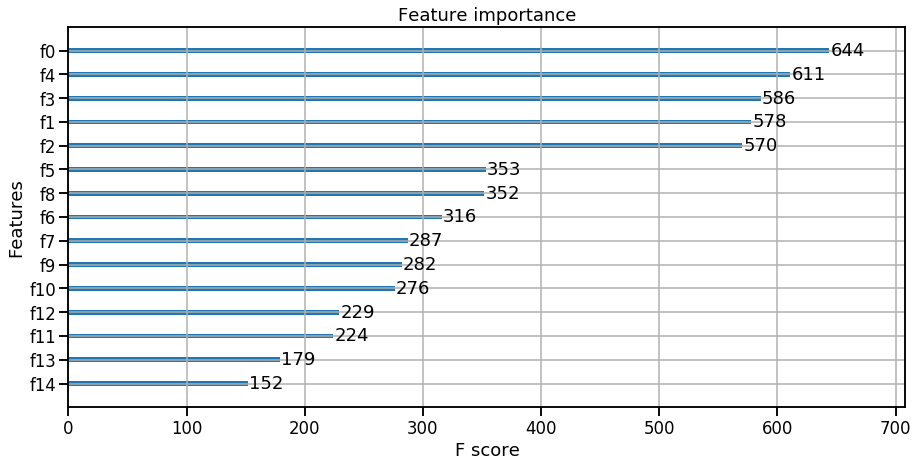
\includegraphics[width=0.8\textwidth]{xgboost_feature_imp}
		\caption{Relative importance for each feature provided by the trained XGBoost model.}
		\label{fig:xgboost_feature_imp}
	\end{adjustwidth}
\end{figure}